
\section{Quantile classifiers for univariate data}
\label{sec:univariate-classifier}

In this section, we review the quantile classifier, a univariate distance-based
classification method.  As noted in Section \ref{sec:intro}, the fundamental
motivation for the family of classifiers proposed in this paper is the result
that for univariate data and under some assumptions, the decision rule based
upon the distances of an observation to the corresponding within-class quantiles
for the optimal choice of quantile levels is the Bayes rule.  The proposed
classifiers for multivariate data are then constructed by considering each
component of the observed data as a 1-dimensional problem, and then aggregating
these most powerful univariate classifiers in some manner to create a
multivariate classifier.  From this perspective, we find it natural to present
our proposed methodology by first considering the application of quantile
classifiers in the univariate setting.

The quantile classifier and the empirically optimal quantile classifier was
introduced in Hennig and Viroli (2016).  For completeness, the notation and
definitions are reintroduced in Sections \ref{sec:quantile-classifier} and
\ref{sec:empirical-classifier}.  In Section
\ref{sec:quantile-classifier-optimality} we present some results for the
quantile classifier in the univariate setting.  A closed-form expression for the
decision boundary for the quantile classifier for a fixed choice of quantile
level is derived, as well as a closed-form solution for the empirical quantile
for a given quantile level.  It is shown that these two results in conjunction
yield a decision rule that can be found in $\bigO(n)$ time, where $n$ is the
number of observations in the training data.  Consistency of both the estimated
optimal quantile level and that of the empirically optimal quantile classifier
is established.  Furthermore, an algorithm is proposed that obtains the decision
rule for the empirically optimal quantile classifier in $\bigO(n^2)$ time.




\subsection{The quantile classifier}
\label{sec:quantile-classifier}

In order to present the quantile classifier, we begin by defining some
terminology.  Consider the check loss (also known as the quantile loss) function
defined as
\begin{align}
  \label{eq:check-loss}
  \rho_\theta(u)
  = \ind(u > 0)\, \theta\, u  + \ind (u \leq 0)\, (1 - \theta)\, (-u)
  = u\, \big[ \theta - \ind(u \leq 0) \big],
\end{align}
for some choice of quantile level $\theta \in (0,1)$.  A plot of the check loss
function for various choices of quantile level is presented in Figure
\ref{fig:quantile-loss}.  This loss function has the important property that for
the $\theta$-th quantile level of a continuous univariate random variable $X$ it
induces the $\theta$-th quantile as the minimizer of the expected distance to
$X$.  That is,
\begin{equation}
  \label{eq:check-loss-min}
  \argmin_q \ev \big[ \rho_\theta (X - q) \big] = F_X^{-1}(\theta),
\end{equation}
for $F_X$ the distribution function of $X$.  Next, consider two populations
$\Pi_0$ and $\Pi_1$ with corresponding distribution functions $F_0$ and $F_1$ on
$\mathbb{R}$.  We define the quantile distance of a point $z$ to the
population's $\theta$-th quantile as
\begin{equation}
  \label{eq:phi}
  \Phi_i(z, \theta) = \rho_{\theta}\Big(z - F_i^{-1}(\theta)\Big),
  \hspace{5mm} i = 0, 1.
\end{equation}
It will also be convenient later to define for fixed $\theta$,
\begin{equation}
  \label{eq:F-order-stats}
  F_{(0)}^{-1}(\theta) = \min\Big\{ F_0^{-1}(\theta),~ F_1^{-1}(\theta) \Big\}
  \hspace{5mm} \text{and} \hspace{5mm}
  F_{(1)}^{-1}(\theta) = \max\Big\{ F_0^{-1}(\theta),~ F_1^{-1}(\theta) \Big\}.
\end{equation}
Next, the difference of the quantile distances of a point $z$ to the populations'
$\theta$-th quantiles is defined as
\begin{equation}
  \Lambda\,(z, \theta) = \Phi_1(z, \theta) - \Phi_0(z, \theta).
\end{equation}
With these definitions in hand, the $\theta$-th quantile-based classifier is
defined as follows.
\begin{equation}
  \label{eq:quantile-classifier}
  \text{For an observation $z$, classify to:} \hspace{5mm} \left\{ 
    \begin{array}{lcl}
      \Pi_0, & & \text{if} \hspace{3mm}\Lambda\,(z, \theta) > 0 \\[0ex]
      \Pi_1, & & \text{otherwise}
    \end{array} .
  \right.
\end{equation}
Finally, let $Z$ be a random variable with a prior probability $\pi_0$ of being
a member of population $\Pi_0$, and $\pi_1 = 1 - \pi_0$ the prior probability of
being a member of population $\Pi_1$.  Then the probability of correctly
classifying an observed realization of $Z$ by the $\theta$-th quantile
classifier is given by
\begin{equation}
  \label{eq:theoretical-rate}
  \Psi(\theta) =
  \pi_0 \int \ind\Big( \Lambda(z, \theta) > 0 \Big)\, dP_0(z) +
  \pi_1 \int \ind\Big(\Lambda(z, \theta) \leq 0 \Big)\, dP_1(z).
\end{equation}
The expression given in (\ref{eq:theoretical-rate}) has the appealing property
that for the optimal choice of quantile level $\theta$ the classification rate
is equal to that of the Bayes classifier.  This result is formally stated as
Theorem \ref{thm:quantile-classifier-is-bayes}.

\begin{figure}[ht]
  \caption[Quantile loss function]{Plots of the check loss function for various
    choices of quantile levels.}
  \label{fig:quantile-loss}
  \vspace{5mm}

  \begin{minipage}[t]{0.33\linewidth}
    \centering
    \includegraphics{check-loss-0-1}
  \end{minipage}
  \begin{minipage}[t]{0.33\linewidth}
    \centering
    \includegraphics{check-loss-0-5}
  \end{minipage}
  \begin{minipage}[t]{0.33\linewidth}
    \centering
    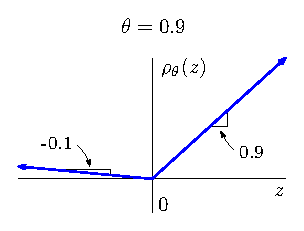
\includegraphics{check-loss-0-9}
  \end{minipage}
  
\end{figure}


\begin{figure}[p]
  \caption[cccc]{Example within-class quantile distances and differences for two
    choices of quantiles.  The left column and right column show the quantile
    distances and differences for the 0.25-th and 0.75th quantile levels,
    respectively (and for arbitrary choices of $F_0^{-1}(\theta)$ and
    $F_1^{-1}(\theta)$).  In all figures the quantile classifier decision rule
    boundary is denoted as $\tau$.  The first row plots the quantile distances
    $\Phi_{(0)}$ and $\Phi_{(1)}$.  The second and third rows plot the quantile
    distance differences for two cases.  In the first case,
    $F_0^{-1}(\theta) < F_1^{-1}(\theta)$, while in the second case
    $F_0^{-1}(\theta) > F_1^{-1}(\theta)$.}
  \label{fig:phi-lambda}
  \vspace{5mm}
  
  \begin{minipage}[t]{0.49\linewidth}
    \centering
    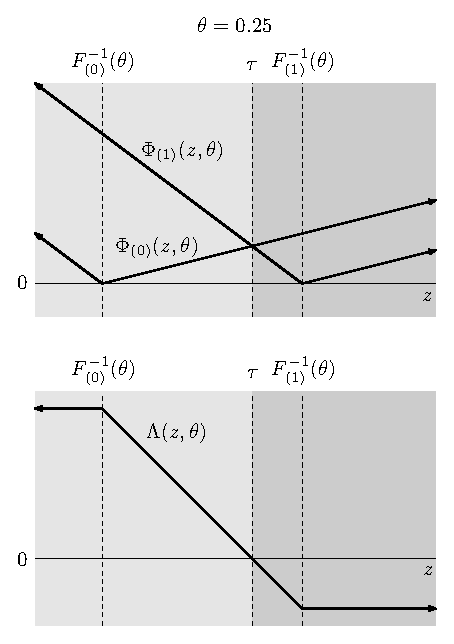
\includegraphics{phi-lambda-0-25}
  \end{minipage}
  \begin{minipage}[t]{0.49\linewidth}
    \centering
    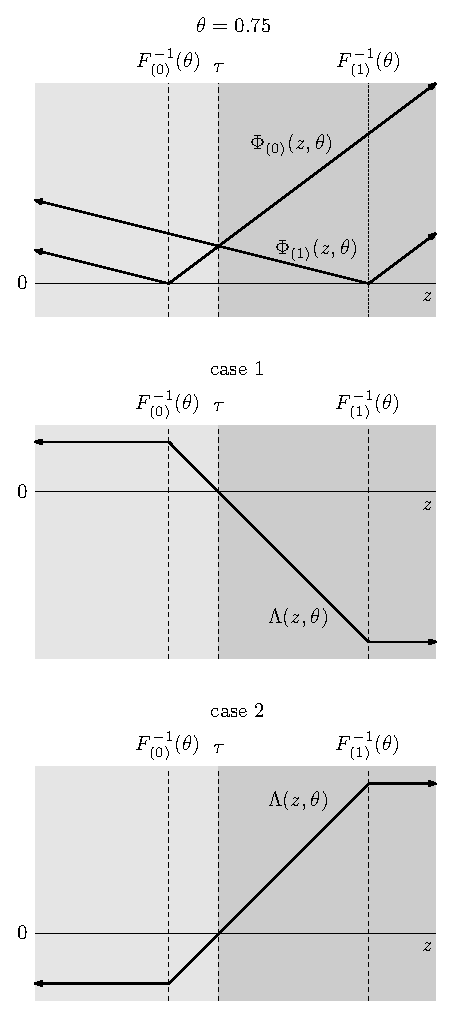
\includegraphics{phi-lambda-0-75}
  \end{minipage}
  
\end{figure}

% \begin{theorem}
%   \label{thm:quantile-classifier-is-bayes}
%   Consider two populations $\Pi_0$ and $\Pi_1$ with corresponding density
%   functions $f_0$ and $f_1$ such that $f_0$ and $f_1$ are nonzero on the same
%   domain.  Let $Z$ be a random variable with a prior probability $\pi_0$ of
%   being a member of population $\Pi_0$, and $\pi_1 = 1 - \pi_0$ the prior
%   probability of being a member of population $\Pi_1$.  Further assume that
%   there is a point $z^{*}$ with $\pi_0\, f_0(z^{*}) = \pi_1\, f_1(z^{*})$ so
%   that $\pi_0\, f_0(z) < \pi_1\, f_1(z)$ for $z$ on one size of $z^{*}$, and
%   $\pi_0\, f_0(z) > \pi_1\, f_1(z)$ on the other side of $z^{*}$.  Then the
%   quantile classifier for an observed realization of $Z$ using the optimal
%   choice of quantile level achieves the Bayes rule classification probability.
% \end{theorem}

% \begin{proof}
%   This result and proof were given as Lemma 2 in \cite{hennig2016}.
% \end{proof}


% Next, let $x_1, \dots, x_n$ be samples from a population with a probability
% density on $\mathbb{R}$.  Then we define the $\theta^{\text{th}}$ empirical
% quantile for the population to be given by minimizer of the sample version of
% equation (\ref{eq: check loss min}) defined by:

% Next, let $\Pi_0$ and $\Pi_1$ be
% two populations with probability densities $P_0$ and $P_1$ on $\mathbb{R}$.
% Consider observations $x_{0, 1}, \dots, x_{0, n_0}$ sampled from population
% $\Pi_0$ and observations $x_{1, 1}, \dots, x_{1, n_1}$ sampled from population $\Pi_1$.
% Then we define $\widehat{F}^{-1}_i (\theta)$ to be the $\theta^{\text{th}}$
% empirical quantile for population $\Pi_i$, where
% \begin{equation}
%   \label{eq: empirical quantile}
%   \widehat{F}^{-1} (\theta) = \argmin_q \left\{ \theta \sum_{ x_{i} > q } |x_{i} - q| ~+~
%     (1 - \theta) \sum_{ x_{i} \leq q } |x_{i} - q| \right\}.
% \end{equation}
% Thus, the empirical quantile is the the minimizer of the sample version of
% equation (\ref{eq: check loss min}).  Finally, let $z$ be a new observation.
% Then classify $z$ to
% \begin{equation}
%   \label{eq: distance classifier}
%   \left\{ 
%     \begin{array}{lcl}
%       \Pi_0, & & \text{if} \hspace{3mm} \rho_{\theta} \left( z - \widehat{F}^{-1}_1 (\theta) \right) ~-~
%                  \rho_{\theta} \left( z - \widehat{F}^{-1}_0 (\theta) \right) ~>~ 0 \\[0ex]
%       \Pi_1, & & \text{otherwise}
%     \end{array}
%   \right.
% \end{equation}
% Conceptually, classify the observation to the population for which it has the
% smaller quantile distance to from the $\theta^{\text{th}}$ quantile.

% To use the classification rule given in equation (\ref{eq: distance classifier})
% in practice, it remains to select a choice of quantile level $\theta$.  In the
% following sections we consider two approaches for selecting the quantile level,
% with an eye towards the extension of the classification rule to the multivariate
% setting.


\subsection{The empirically optimal quantile classifier}
\label{sec:empirical-classifier}

Next we introduce some terminology with which to introduce the sample version of
the optimal quantile classifier.  Let $x_1, \dots, x_m$ be samples from a
population with a probability density on $\mathbb{R}$.  Then we define the
$\theta$-th empirical quantile for the population to be given by any minimizer
of the sample version of equation (\ref{eq:check-loss-min}), defined by
\begin{equation}
  \label{eq:empirical-quantile}
  \hat{F}^{-1} (\theta) = \argmin_q \left\{
    \theta \sum_{ x_{i} > q } |x_{i} - q| ~+~
    (1 - \theta) \sum_{ x_{i} \leq q } |x_{i} - q|
  \right\}.
\end{equation}
It is interesting to note that we can view equation
(\ref{eq:empirical-quantile}) as the solution to a quantile regression problem
introduced in \cite{koenker1978}, where the $x_i$'s correspond to the response
variables, and $q$ is a single regression coefficient corresponding to predictor
data with only an intercept term and no other covariates.  In light of this
fact, we may utilize any of the theory developed in the quantile regression
literature to solve this minimization problem.  However, it turns out that there
is a simple closed-form solution available for this particular special case of
quantile regression, which is presented as Lemma \ref{lem:empirical-quantlev}.

Having defined the $\theta$-th empirical quantile for the population, it follows
that the empirical difference of the quantile distances of a point $z$ to the
population's $\theta$-th quantiles is defined as
\[
  \Lambda_n (z, \theta) = \rho_{\theta}\Big(z - \hat{F}_{1n}^{-1}(\theta)\Big) -
  \rho_{\theta}\Big(z - \hat{F}_{0n}^{-1}(\theta)\Big),
\]
where $\hat{F}_{1n}$ is the estimate of the $\theta$-th quantile level of
population $\Pi_1$ based on the samples in $x_1, \dots, x_n$ that came from
population $\Pi_1$, and similarly for $\hat{F}_{0n}$.  Let $n_0$ and $n_1$
be the number of observations from $\Pi_0$, and $\Pi_1$, respectively.  Then we
further define the observed rate of correct classification for the $\theta$-th
quantile as
\begin{align}
  \begin{split}
    \Psi_n(\theta)
    &= \frac{n_0}{n_0 + n_1} \left[
      \frac{1}{n_0} \sum_{x_i \in \Pi_0}
      \mathbbm{1}\Big( \Lambda_n(x_i, \theta) > 0 \Big)
    \right] +
      \frac{n_1}{n_0 + n_1} \left[
        \frac{1}{n_1} \sum_{x_i \in \Pi_1}
        \mathbbm{1}\Big( \Lambda_n(x_i, \theta) \leq 0 \Big)
      \right] \\[1ex]
    &= \frac{1}{n} \left[
      \sum_{x_i \in \Pi_0} \mathbbm{1}\Big( \Lambda_n(x_i, \theta) > 0 \Big) +
      \sum_{x_i \in \Pi_1} \mathbbm{1}\Big( \Lambda_n(x_i, \theta) \leq 0 \Big)
    \right].
  \end{split}
\end{align}
Finally, define the empirically optimal quantile classifier to be any solution
to the equation
\begin{equation}
  \label{eq:theta-hat}
  \hat{\theta}_n = \argmax_{\theta \in T} \Psi_n(\theta),
\end{equation}
where $T = [\delta, 1 - \delta]$ for some small positive constant $\delta$.  The
restriction of quantile levels to the set $T$ is in order to guarantee at least
one optimal value of $\theta$ for the theoretical quantile classifier, otherwise
the optimal quantile level may converge to 0 or 1 in the limit.



% \vspace{10mm} Let $z$ be a univariate observation with a prior
% probability $\pi_0$ of being a member of class 0, and $1 - \pi_0 = \pi_1$ the
% prior probability of being a member of class 1.  Then for quantile level
% $\theta$, define
% \[
%   \rho\,(z, \theta) = \rho_{\theta}\Big(z,\, F_1^{-1}(\theta)\Big) -
%   \rho_{\theta}\Big(z,\, F_0^{-1}(\theta)\Big)
% \]
% Then the probability of a correct classification by the quantile classifier is
% given by
% \begin{equation}
%   \label{eq: theoretical rate}
%   \pi_0 \int \ind\Big( \rho(z, \theta) > 0 \Big)\, dP_0(z) + \pi_1 \int \ind\Big(
%   \rho(z, \theta) \leq 0 \Big) \,dP_1(z)
% \end{equation}
% The expression given in (\ref{eq:theoretical-rate}) has the appealing property
% that for the optimal choice of quantile level $\theta$ the classification rate is
% equal to that of the Bayes classifier.  Thus, to select the quantile level for
% the classification rule given by (\ref{eq:distance-classifier}), one approach
% is to select the empirically optimal choice of $\theta$, as determined by
% leave-one-out cross validation.  To give the definition of this estimator, we
% first describe the setting and introduce some preliminary definitions.

% Consider observations $x_{0, 1}, \dots, x_{0, n_0}$ sampled from population
% $\Pi_0$ and observations $x_{1, 1}, \dots, x_{1, n_1}$ sampled from population $\Pi_1$.
% Then we define
% \[
%   \widehat{\rho}(z, \theta) = \rho_{\theta}\Big(z,\,
%   \widehat{F}_1^{-1}(\theta)\Big) - \rho_{\theta}\Big(z,\,
%   \widehat{F}_0^{-1}(\theta)\Big)
% \]
% where $\widehat{F}_i^{-1}(\theta)$ is estimated from
% $x_{i,1}, x_{i,2}, \dots, x_{i,n_i},~ i = 1, 2$.  Further define
% $\widehat{\rho}_{-x_{i, j}} (z, \theta)$ to be as above, but where
% $\widehat{F}_i^{-1}(\theta)$ is estimated from the data after leaving out the
% $x_{i, j}$ observation (and the estimate of the comparison quantile is
% obtained using the full set of observations from that class).  Then we define
% the empirically optimal quantile level to be given by
% \begin{align}
%   \begin{split}
%     \widehat{\theta^{\text{opt}}}
%     &= \argmax_{\theta \in \{\theta_1, \dots, \theta_K\}} \left\{ \frac{n_0}{n_0 + n_1} \left[ \frac{1}{n_0} \sum_{z \in \Pi_0} \mathbbm{1}\Big( \widehat{\rho}_{-z}(z, \theta) > 0 \Big)  \right] +
%       \frac{n_1}{n_0 + n_1} \left[ \frac{1}{n_1} \sum_{z \in \Pi_1} \mathbbm{1}\Big( \widehat{\rho}_{-z}(z, \theta) \leq 0 \Big)  \right] \right\} \\[1ex]
%     &= \argmax_{\theta \in \{\theta_1, \dots, \theta_K\}} \left\{ \sum_{z \in \Pi_0} \mathbbm{1}\Big( \widehat{\rho}_{-z}(z, \theta) > 0 \Big) +
%       \sum_{z \in \Pi_1} \mathbbm{1}\Big( \widehat{\rho}_{-z}(z, \theta) \leq 0 \Big) \right\}
%   \end{split}
% \end{align}
% for $\theta_1, \dots, \theta_K$ a grid of quantile levels from which to compare.
% Conceptually, $\widehat{\theta^{\text{opt}}}$ is chosen to be the optimizer of
% the sample version of the theoretical optimizer given in equation
% (\ref{eq:theoretical-rate}).

% \begin{editornote}
%   This seems like a reasonable strategy and we have shown empirically that good
%   estimates for the optimal quantile level can be found for a moderate sample
%   size (see project update pdf for 2016-07-01).  However it does have some
%   drawbacks:
  
%   \begin{itemize}
%   \item adds computational burden to the method
%   \item eats up our sample size in that we should set aside training data to
%     train on the quantile estimates
%   \item practical issues with small sample sizes: seems unstable.  Depending on
%     the sample size and the proportion of observations, one class can end up
%     with just a handful or even no observations for a particular class.
%   \end{itemize}
  
% \end{editornote}


% \subsection{Choice of quantile level: distance-based}

% Another approach to selecting the quantile level for the classification rule
% given in expression (\ref{eq: distance classifier}) is based on comparing the
% distances between the quantiles for each class.  Intuitively, the quantiles with
% greater differences between the classes may contain more information in
% discriminating new observations through a comparison of their quantile distances
% to the quantile.  In this section we consider a class of composite
% distance-based quantile levels.

% One major drawback to selecting quantile levels based on a comparison of the
% distances between quantiles is the following.  Consider as an example the case
% where the observations are drawn from populations $\Pi_0$ and $\Pi_1$ such that
% the densities for the populations are $\normal(\mu_0, 1)$ and
% $\normal(\mu_1, 1)$, respectively.  Then
% $\big|F_1^{-1}(\theta) - F_0^{-1}(\theta)\big| = |\mu_1 - \mu_0|$ for all $\theta$. In
% this particular example, the optimal choice of quantile level is 0.5; however,
% when using a distance-based approach to selecting the quantile there is no
% meaningful information from which to make a decision, a clearly undesirable
% property.  However, when extending the classification rule to the multivariate
% setting, there is not a direct connection between the classification problem
% based on one variable and the classification problem drawing information from
% all of the variables, and in practice we may achieve better performance with
% this approach in some settings.

% We propose a class of composite distance-based quantile levels constructed as
% follows.  Consider a grid of quantile levels $\theta_1, \dots, \theta_K$.  Define
% \[
%   d_k = \left| \widehat{F}^{-1}_1 (\theta_k) - \widehat{F}^{-1}_0
%     (\theta_k) \,\right|, \hspace{5mm} k = 1, \dots, K
% \]
% Then a class of component-wise quantile weights is defined as
% \begin{equation}
%   w_k = \frac{ (d_k - \epsilon)_{+}^{\nu} }{ \sum_{\ell = 1}^K (d_{\ell}
%     - \epsilon)_{+}^{\nu} }, \hspace{5mm} k = 1, \dots, K.
% \end{equation}
% where $\nu$ and $\epsilon$ are nonnegative tuning parameters.
% % Various choices
% % of $\nu$ and $\epsilon$ lead to special cases such as
% % \begin{itemize}
% % \item $w_k = 1 / K$
% % \item $\displaystyle w_k = \frac{ (d_k - \epsilon)_+ }
% %   { \sum_{\ell=1}^K (d_{\ell} - \epsilon)_+ }$
% % \item $\displaystyle w_k = \frac{ d_{k}^2 }{ \sum_{\ell=1}^K d_{\ell}^2 }$
% % \end{itemize}
% When using composite quantile levels we write the classifier as follows.  For
% new observation $z$, classify to
% \begin{equation}
%   \label{eq: composite classifier}
%   \left\{ 
%     \begin{array}{lcl}
%       \Pi_0, & & \displaystyle \text{if} \hspace{3mm} \sum_{k=1}^K w_{jk}\,
%                  \bigg\{ \rho_{\theta_k} \left( z - \widehat{F}^{-1}_1 (\theta_k) \right) -
%                  \rho_{\theta_k} \left( z - \widehat{F}^{-1}_0 (\theta_k) \right) \bigg\}
%                  ~>~ 0 \\[2ex]
%       \Pi_1, & & \text{otherwise} \\[1ex]
%     \end{array}
%   \right.
% \end{equation}


% \subsection{Optimal quantile level estimation properties}
% \label{sec: opt quantile est}

% In this section we investigate the finite-sample properties of the leave-one-out
% cross validation approach for estimating the classification rate as a function
% of quantile level.
% \\
% ****  TODO: rework this section if we think it belongs in the paper.  *****
% \\
% \includegraphics[width=1\textwidth]{../../R_Scratch/Plots/Case1.pdf}



\subsection{Optimality and consistency of the quantile classifier}
\label{sec:quantile-classifier-optimality}

With the definitions for the quantile classifier in place, we now provide some
of its properties.  We begin with the fundamental result for the motivation of
the paper, that the quantile classifier achieves the Bayes rule classification
rate for the optimal choice of quantile level.  The following result is due to
\cite{hennig2016}.

\begin{proposition}
  \label{thm:quantile-classifier-is-bayes}
  Consider two populations $\Pi_0$ and $\Pi_1$ with corresponding density
  functions $f_0$ and $f_1$ such that $f_0$ and $f_1$ are nonzero on the same
  domain.  Let $Z$ be a random variable with a prior probability $\pi_0$ of
  being a member of population $\Pi_0$, and $\pi_1 = 1 - \pi_0$ the prior
  probability of being a member of population $\Pi_1$.  Further assume that
  there is a point $z^{*}$ with $\pi_0\, f_0(z^{*}) = \pi_1\, f_1(z^{*})$ so
  that $\pi_0\, f_0(z) < \pi_1\, f_1(z)$ for $z$ on one size of $z^{*}$, and
  $\pi_0\, f_0(z) > \pi_1\, f_1(z)$ on the other side of $z^{*}$.  Then the
  quantile classifier for an observed realization of $Z$ using the optimal
  choice of quantile level achieves the Bayes rule misclassification
  probability.
\end{proposition}

Having established the theoretical optimality of the quantile classifier, we now
consider the consistency of the empirical version.  The following result is
essentially a special case of a theorem presented in \cite{hennig2016}.  For
this result, we will need the following assumptions.  Let $\delta$ be a small
positive constant.
\begin{enumerate}[label=\emph{Assumption \arabic*.}, align=left]
\item $F_i^{-1}$ is a continuous function of
  $\theta,~ i=0,1$.
\item $\prob\Big( \Lambda(Z, \theta) = 0 \Big) = 0$ for all
  $\theta \in [\delta, 1 - \delta]$.
\item There is a unique $\tilde{\theta}$ that satisfies $\tilde{\theta} =
  \argmax_{\theta \in T} \Psi(\theta)$.
\end{enumerate}

\begin{lemma}
  \label{lem:univariate-consistency}
  Let $\tilde{\theta}$ be a solution to
  $\tilde{\theta} = \argmax_{\theta \in T} \Psi(\theta)$.  Under Assumptions 1
  and 2, it follows that
  $\Psi(\hat{\theta}_n) \stackrel{p}{\longrightarrow} \Psi(\tilde{\theta})$.
  Furthermore, under Assumptions 1, 2, and 3, it follows that
  $\hat{\theta}_n \stackrel{p}{\longrightarrow} \tilde{\theta}$.
\end{lemma}

\begin{proof}
  The fact that
  $\Psi(\hat{\theta}_n) \stackrel{p}{\longrightarrow} \Psi(\tilde{\theta})$ is a
  special case of Theorem 1 in \cite{hennig2016} for a feature-space of
  dimension 1.  Furthermore, during the proof of that theorem it was shown that
  under Assumptions 1 and 2, $\Psi$ is a continuous function of $\theta$.  To
  show that $\hat{\theta}_n \stackrel{p}{\longrightarrow} \tilde{\theta}$
  suppose that the claim doesn't hold.  Then there exists an $\epsilon > 0$ and
  $\delta > 0$ such that for all $N \in \mathbb{N}$, there exists an $n \geq N$
  such that
  \begin{equation*}
    \prob\Big(
    \big| \hat{\theta}_n - \tilde{\theta} \big|
    > \epsilon \Big)
    \geq \delta.
  \end{equation*}
  Now, because $\Psi$ is continuous and $\Psi(\tilde{\theta})$ is a unique
  maximum, it follows that we can find $\nu > 0$ such that
  \begin{equation*}
    \min \left\{
      \big| \Psi(\Tilde{\theta} - \epsilon) - \Psi(\tilde{\theta}) \big|\,,
      \hspace{2mm}
      \big| \Psi(\Tilde{\theta} + \epsilon) - \Psi(\tilde{\theta}) \big|
    \right\} \geq \nu.
  \end{equation*}
  Therefore, for all $N \in \mathbb{N}$, there exists an $n \geq N$ such that
  \begin{equation*}
    \prob\Big(
    \big| \Psi(\hat{\theta}_n) - \Psi(\tilde{\theta}) \big|
    \geq \nu \Big) \geq
    \prob\Big(
    \big| \hat{\theta}_n - \tilde{\theta} \big|
    \geq \epsilon \Big)
    \geq \delta.
  \end{equation*}
  But this is in contradiction to the fact that
  $\Psi(\hat{\theta}_n) \stackrel{p}{\longrightarrow} \Psi(\tilde{\theta})$.
\end{proof}




\subsection{Decision rule calculation}
\label{sec:empirical-quantile-classifier-results}

So it is established that the classification rate of the empirically optimal
quantile classifier converges to the classification rate of the true optimal
quantile classifier.  Next, we investigate the practical considerations of
calculating the empirically optimal quantile classifier.  Let us define
$\Phi_{(0)}(z, \theta) = \rho_{\theta}\left(z - F_{(0)}^{-1}(\theta)\right)$ and
$\Phi_{(1)}(z, \theta) = \rho_{\theta}\left(z - F_{(1)}^{-1}(\theta)\right)$,
and let $\Pi_{(0)}$ and $\Pi_{(1)}$ be such that
$F_{\Pi_{(0)}}^{-1}(\theta) < F_{\Pi_{(1)}}^{-1}(\theta)$.

\begin{lemma}
  \label{lem:decision-boundary}
  If $F_{(0)}^{-1}(\theta) \ne F_{(1)}^{-1}(\theta)$, then the quantile
  classifier defined in equation (\ref{eq:quantile-classifier}) can be
  equivalently expressed as follows.
  \begin{equation}
    \label{eq:alt-quantile-classifier}
    \text{For an observation $z$, classify to:} \hspace{5mm} \left\{ 
      \begin{array}{lcl}
        \Pi_{(0)}, & & z ~<~ \theta F_{(0)}^{-1}(\theta) +
                       (1 - \theta)\, F_{(1)}^{-1}(\theta) \\[1ex]
        \Pi_{1}, & & z ~=~ \theta F_{(0)}^{-1}(\theta) +
                       (1 - \theta)\, F_{(1)}^{-1}(\theta) \\[1ex]
        \Pi_{(1)}, & & \textup{otherwise}
      \end{array}
    \right.
  \end{equation}
\end{lemma}

\begin{proof}
  Suppose $F_{(0)}^{-1}(\theta) \ne F_{(1)}^{-1}(\theta)$.  It is clear
  (e.g. see Figure \ref{fig:phi-lambda}) that $\Phi_{(0)}(z, \theta)$ is
  equal to $\Phi_{(1)}(z, \theta)$ at exactly one point, say $\tau$, and that
  the following holds:
  \begin{equation*}
    \left\{
      \begin{array}{lll}
        \Phi_{(0)}(z, \theta) < \Phi_{(1)}(z, \theta), & & z < \tau \\[1ex]
        \Phi_{(0)}(z, \theta) = \Phi_{(1)}(z, \theta), & & z = \tau \\[1ex]
        \Phi_{(0)}(z, \theta) > \Phi_{(1)}(z, \theta), & & z > \tau \\
      \end{array}
    \right.
  \end{equation*}
  Furthermore, we can infer that
  $F_{(0)}^{-1}(\theta) < \tau < F_{(1)}^{-1}(\theta)$.  Setting the loss
  functions equal for $z$ in this interval yields:
  \begin{align*}
    & \Phi_{(0)}(z, \theta) \stackrel{\mathit{set}}{=} \Phi_{(1)}(z, \theta) \\
    & \hspace{5mm} \Longleftrightarrow \hspace{5mm}
      \ind\!\! \left(z > F_{(0)}^{-1}(\theta)\right) \theta
      \left(z - F_{(0)}^{-1}(\theta)\right) +
      \ind\!\! \left(z \leq F_{(0)}^{-1}(\theta)\right) (1 - \theta)
      \left(F_{(0)}^{-1}(\theta) - z\right) \\
    & \hspace{25mm} =
      \ind\!\! \left(z > F_{(1)}^{-1}(\theta)\right) \theta
      \left(z - F_{(1)}^{-1}(\theta)\right) +
      \ind\!\! \left(z \leq F_{(1)}^{-1}(\theta)\right) (1 - \theta)
      \left(F_{(1)}^{-1}(\theta) - z\right) \\
    & \hspace{5mm} \Longleftrightarrow \hspace{5mm}
      \theta \left(z - F_{(0)}^{-1}(\theta)\right) =
      (1 - \theta) \left(F_{(1)}^{-1}(\theta) - z\right) \\
    & \hspace{5mm} \Longleftrightarrow \hspace{5mm}
      z = \theta\, F_{(0)}^{-1}(\theta) + (1 - \theta)\, F_{(1)}^{-1}(\theta).
  \end{align*}
  It can then be verified that $\Phi_{(0)}(z, \theta) < \Phi_{(1)}(z, \theta)$
  corresponds to classifying $z$ to $\Pi_{(0)}$ and that
  $\Phi_{(0)}(z, \theta) > \Phi_{(1)}(z, \theta)$ corresponds to classifying $z$
  to $\Pi_{(1)}$.  Combining these facts yields the desired result.
\end{proof}
It is interesting to note that the decision rule boundary lies on the line
segment between $F_0^{-1}(\theta)$ and $F_1^{-1}(\theta)$, with the location of
the point on the line determined by the quantile level.  The next result
characterizes the solution set for the empirical quantile level estimator.

\begin{lemma}
  \label{lem:empirical-quantlev}
  Let $x_1, \dots, x_m$ be points on $\mathbb{R}$.  Then a solution to equation
  (\ref{eq:empirical-quantile}) providing the $\theta$-th empirical quantile for
  $x_1, \dots, x_m$ is given by $\lceil m \theta \rceil$-th largest value of the
  $x_i$.
\end{lemma}

\begin{proof}
  % 
We can write the minimization problem
\begin{equation*}
  \min_q \left\{
    \theta \sum_{ x_{i} > q } |x_{i} - q| ~+~
    (1 - \theta) \sum_{ x_{i} \leq q } |x_{i} - q|
  \right\}
\end{equation*}
equivalently as
% \begin{align*}
%   &\min_{q^{+}, q^{-}, \vec{u}, \vec{v}} \left\{
%     \theta \sum_{i=1}^m u_i ~+~
%     (1 - \theta) \sum_{i=1}^m v_i
%   \right\} \\[2ex]
%   & \text{subject to} \hspace{3mm}
%   x_i - (q^{+} - q^{-}) = u_i - v_i, \hspace{5mm} i = 1, \dots, m \\[2ex]
%   & q^{+} \geq 0,~ q^{-} \geq 0,~ \vec{u} \geq \vec{0},~ \vec{v} \geq 0
% \end{align*}
\begin{equation*}
  \arraycolsep=5mm
  \begin{array}{ll}
    \displaystyle
    \minimize_{q^{+}, q^{-}, \vec{u}, \vec{v}}
    & \theta \sum_{i=1}^m u_i ~+~
      (1 - \theta) \sum_{i=1}^m v_i \\[2ex]
    \text{subject to}
    & x_i - (q^{+} - q^{-}) = u_i - v_i, \hspace{5mm} i = 1, \dots, m \\[2ex]
    & q^{+} \geq 0,~ q^{-} \geq 0,~ \vec{u} \geq \vec{0},~ \vec{v} \geq \vec{0} \\
  \end{array}
\end{equation*}
which is seen to be a linear programming problem in standard form.  By rewriting
the equality condition as $q^{+} - q^{-} + u_i - v_i = x_i$ for $i=1, \dots, m$,
we can express the equality condition in matrix form as
\begin{equation*}
  \begin{bmatrix}
    1      & -1     & 1 &        &   & -1 &        &    \\
    \vdots & \vdots &   & \ddots &   &    & \ddots &    \\
    1      & -1     &   &        & 1 &    &        & -1 \\
  \end{bmatrix}
  % \begin{bmatrix}
  %   q^{+} \\ q^{-} \\ u_{1} \\ \vdots \\ u_m \\ v_1 \\ \vdots \\ v_m \\
  % \end{bmatrix}
  \begin{bmatrix}
    q^{+} \\ q^{-} \\ \vec{u} \\ \vec{v} \\
  \end{bmatrix}
  =
  \begin{bmatrix}
    x_1 \\ \vdots \\ x_m \\
  \end{bmatrix}.
\end{equation*}
% \begin{equation*}
%   \begin{bmatrix}
%     1      & -1     & 1         &        &  \bigDown{0} & -1        &        & \bigDown{0} \\
%     \vdots & \vdots &           & \ddots &              &           & \ddots &             \\
%     1      & -1     & \bigUp{0} &        & 1            & \bigUp{0} &        & -1          \\
%   \end{bmatrix}
% \end{equation*}
% \begin{equation*}
%   \begin{bmatrix}
%     1      & -1     & &         &  & &          & \\
%     \vdots & \vdots & & \vec{I} &  & & -\vec{I} & \\
%     1      & -1     & &         &  & &          & \\
%   \end{bmatrix}
% \end{equation*}
% \begin{equation*}
%   \begin{bmatrix}
%     1      & -1     & 1      & 0      & \dots  & 0       & -1     &        &    \\
%     \vdots & \vdots & 0      & \ddots & \ddots & \vdots  &  0     & \ddots & \\
%     \vdots & \vdots & \vdots & \ddots & \ddots & 0       & \vdots & \ddots & \ddots &    \\
%     1      & -1     & 0      & \dots  & 0      & 1       &  0     & \dots  &  0     & -1 \\
%   \end{bmatrix}
% \end{equation*}
Recall that a solution for $(q^{+}, q^{-}, \vec{u}, \vec{v})$ is a basic
solution if and only if there exist indices $B(1), \dots, B(m)$ such that both
(i) the columns of the coefficient matrix with column indices subset by
$B(1), \dots, B(m)$ are linearly independent, and (ii) if an element of
$(q^{+}, q^{-}, \vec{u}, \vec{v})$ does not correspond to one of
$B(1), \dots, B(m)$ then the element must have a value of 0.

We can see that in order to have independent columns from the coefficient
matrix, then for each $i$, no more than one of the columns corresponding to
either $u_i$ or $v_i$ can have an index in $B(1), \dots, B(m)$, and additionally
no more than one of the columns corresponding to either $q^{+}$ or $q^{-}$ can
have an index in $B(1), \dots, B(m)$.  Furthermore, we note that if we have one
column corresponding to $q^{+}$ or $q^{-}$, and one column corresponding to
either $u_i$ or $v_i$ for each $i$, then we have $m + 1$ columns, which is still
one column too many.  Thus we see that there must be either (i) exactly one
column corresponding to either $u_i$ or $v_i$ for each $i$ and no columns
corresponding to either $q^{+}$ or $q^{-}$, or (ii) exactly one column
corresponding to either $u_i$ or $v_i$ for each $i$ less one and exactly one
column corresponding to either $q^{+}$ or $q^{-}$.

% Next we notice that if we include a column corresponding to $q^{+}$ or $q^{-}$,
% then the solution for the corresponding coefficient is either the value of $x_i$
% or $-x_i$, and where the index $i$ corresponds to the only $i$ without a column
% corresponding to either $u_i$ or $v_i$.  Then each

Furthermore, we can infer that if a column corresponding to $q^{+}$ or $q^{-}$
has an index in $B(1), \dots, B(m)$ and the solution is feasible (i.e. $q^{+}$
and $q^{-}$ are both nonnegative), then $q^{+} = (x_i)_{+}$ and
$q^{-} = (-x_i)_{+}$, where the index $i$ corresponds to the only $i$ without a
column corresponding to either $u_i$ or $v_i$, and $(z)_{+} = \max(0, z)$.  Let
$q = q^{+} - q^{-}$, then it follows that a feasible solution for any $j \ne i$
has $u_i = (x_i - q)_{+}$ and $v_i = (q - x_i)_{+}$.  This leads to a set of
basic feasible solutions given by $q \in \{x_1, \dots, x_m\}$.  One last basic
feasible solution is given for $q = 0$ with $u_i = (x_i)_{+}$ and
$v_i = (-x_i)_{+}$ for all $i$.

Next we aim to find the minimizing basic feasible solution.  Suppose that
$\lceil \theta m \rceil = k$ and that $\ell < k$, and let $q = x_k$ and
$q^{\prime} = x_{\ell}$.  Then comparing the objective function evaluated at $q$
and $q^{\prime}$, we have
\begin{align*} 
  \left\{ \theta \sum_{i=\ell+1}^m \right.
  & (x_i - q^{\prime}) +
    \left. (1 - \theta) \sum_{i=1}^{\ell} (q^{\prime} - x_i) \right\} -
    \left\{ \theta \sum_{i=k+1}^m (x_i - q) +
    (1 - \theta) \sum_{i=1}^k (q - x_i) \right\} \\[1ex]
  &= (1 - \theta) \sum_{i=1}^{\ell} \Big\{ (q^{\prime} - x_i) - (q - x_i) \Big\} \\
  &\hspace{8mm}
    + \theta \sum_{i=\ell+1}^k (x_i - q^{\prime})
    - (1 - \theta) \sum_{i=\ell+1}^k (q - x_i) \\
  &\hspace{8mm}
    + \theta \sum_{i=k+1}^m \Big\{ (x_i - q^{\prime})
    - (x_i - q) \Big\} \\[1ex]
  % &= (1 - \theta) \sum_{i=1}^{\ell} \Big\{ (q^{\prime} - x_i) - (q - x_i) \Big\} \\
  % &\hspace{8mm}
  %   + \theta \sum_{i=\ell+1}^k (x_i - q^{\prime})
  %   - (1 - \theta) \sum_{i=\ell+1}^k (q - x_i) \\
  % &\hspace{8mm}
  %   + (1 - \theta) \sum_{i=\ell+1}^k (q^{\prime} - x_i)
  %   - (1 - \theta) \sum_{i=\ell+1}^k (q^{\prime} - x_i) \\
  % &\hspace{8mm}
  %   + \theta \sum_{i=k+1}^m \Big\{ (x_i - q^{\prime})
  %   - (x_i - q) \Big\} \\[1ex]
  &= (1 - \theta) \sum_{i=1}^{\ell} \Big\{ (q^{\prime} - x_i) - (q - x_i) \Big\} \\
  &\hspace{8mm}
    + \theta \sum_{i=\ell+1}^k (x_i - q^{\prime})
    - (1 - \theta) \sum_{i=\ell+1}^k (q - x_i)
    \pm (1 - \theta) \sum_{i=\ell+1}^k (q^{\prime} - x_i) \\
  &\hspace{8mm}
    + \theta \sum_{i=k+1}^m \Big\{ (x_i - q^{\prime})
    - (x_i - q) \Big\} \\[1ex]
  &= -(1 - \theta) \sum_{i=1}^{\ell}\, (q - q^{\prime}) \\
  &\hspace{8mm}
    + \theta \sum_{i=\ell+1}^k (x_i - q^{\prime})
    - (1 - \theta) \sum_{i=\ell+1}^k (q - q^{\prime})
    - (1 - \theta) \sum_{i=\ell+1}^k (q^{\prime} - x_i) \\
  &\hspace{8mm}
    + \theta \sum_{i=k+1}^m (q - q^{\prime}) \\[1ex]
  &= -(1 - \theta) \sum_{i=1}^k\, (q - q^{\prime}) \\
  &\hspace{8mm}
    + \theta \sum_{i=\ell+1}^k (x_i - q^{\prime})
    - (1 - \theta) \sum_{i=\ell+1}^k (q^{\prime} - x_i) \\
  &\hspace{8mm}
    + \theta \sum_{i=k+1}^m (q - q^{\prime}) \\[1ex]
  &= -(1 - \theta) \sum_{i=1}^k\, (q - q^{\prime}) \\
  &\hspace{8mm}
    + \sum_{i=\ell+1}^k (x_i - q^{\prime}) \\
  &\hspace{8mm}
    + \theta \sum_{i=k+1}^m (q - q^{\prime}) \\[1ex]
  & = - (1 - \theta)\, k\, (q - q^{\prime})
    + \sum_{i=\ell+1}^k (x_i - q^{\prime})
    + \theta (m - k) (q - q^{\prime}) \\
  &= \sum_{i=\ell+1}^k (x_i - q^{\prime}) - (k - \theta m) (q - q^{\prime}) \\
  &\geq (x_k - q^{\prime}) - (q - q^{\prime}) \\
  &= x_k - q \\
  &= 0
\end{align*}
The inequality is due to the fact that $x_i \geq q^{\prime}$ for
$i \geq \ell + 1$, and also the fact that $k - \theta m < 1$.  Suppose now that
$\lceil \theta m \rceil = k$ and that $\ell > k$, and let $q = x_k$ and
$q^{\prime} = x_{\ell}$.  Then comparing the objective function evaluated at $q$
and $q^{\prime}$, we have
\begin{align*} 
  \left\{ \theta \sum_{i=\ell+1}^m \right.
  & (x_i - q^{\prime}) +
    \left. (1 - \theta) \sum_{i=1}^{\ell} (q^{\prime} - x_i) \right\} -
    \left\{ \theta \sum_{i=k+1}^m (x_i - q) +
    (1 - \theta) \sum_{i=1}^k (q - x_i) \right\} \\[1ex]
  &= (1 - \theta) \sum_{i=1}^k \Big\{ (q^{\prime} - x_i) - (q - x_i) \Big\} \\
  &\hspace{8mm}
    + \theta \sum_{i=k+1}^{\ell} (x_i - q^{\prime})
    - (1 - \theta) \sum_{i=k+1}^{\ell} (q - x_i) \\
  &\hspace{8mm}
    + \theta \sum_{i=\ell+1}^m \Big\{ (x_i - q^{\prime})
    - (x_i - q) \Big\} \\[1ex]
  &= (1 - \theta) \sum_{i=1}^k\, (q^{\prime} - q) \\
  &\hspace{8mm}
    - \theta \sum_{i=k+1}^{\ell} (q^{\prime} - q)
    + \sum_{i=k+1}^{\ell} (x_i - q) \\
  &\hspace{8mm}
    - \theta \sum_{i=l+1}^m (q^{\prime} - q) \\[1ex]
  % &= (1 - \theta) \sum_{i=1}^k\, (q^{\prime} - q) \\
  % &\hspace{8mm}
  %   + \sum_{i=k+1}^{\ell} (x_i - q) \\
  % &\hspace{8mm}
  %   - \theta \sum_{i=k+1}^m (q^{\prime} - q) \\[1ex]
  &= (1 - \theta) \sum_{i=1}^k\, (q^{\prime} - q)
    + \sum_{i=k+1}^{\ell} (x_i - q)
    - \theta \sum_{i=k+1}^m (q^{\prime} - q) \\
  &= (1 - \theta)\, k\, (q^{\prime} - q)
    + \sum_{i=k+1}^{\ell} (x_i - q)
    - \theta\, (m - k) (q^{\prime} - q) \\
  &= (k - \theta m) (q^{\prime} - q) + \sum_{i=k+1}^{\ell} (x_i - q) \\
  &\geq 0
\end{align*}
There is one basic feasible solution remaining to check, that where $q = 0$.  To
show that this is not the optimal solution except in the case that
$x_{\lceil \theta m \rceil} = 0$, we make the following argument.  Note that if
we add some nonzero value $\tau$ to each $x_i$ and if $q^{*}$ is an optimal
choice for the original problem, then $q^{*} + \tau$ is an optimal choice for
the new problem.  Choose $-\tau$ to be one of the $x_i$ for some $i$: then 0 is
one of the values in the transformed data, which was shown in the previous
results to be no better than the $\lceil \theta m \rceil$-th largest value of
the transformed data, so it follows that the $\lceil \theta m \rceil$-th largest
value is optimal.  Since $\tau$ cannot be better than optimal for the transormed
data, then by the law of the contrapositive 0 cannot be better than optimal for
the original data.




%%% Local Variables:
%%% mode: latex
%%% TeX-master: "cqc_paper"
%%% End:

  The proof is relegated to the supplementary materials.  The result is
  essentially a consequence of the fact that the problem can be cast as a linear
  programming problem where the extreme points of the feasible set are the
  values of the $x_i$.
\end{proof}

\begin{lemma}
  \label{lem:decision-rule-time}
  Obtaining the quantile classifier decision rule boundary for fixed choice of
  quantile level is an $\bigO(n)$ operation.
\end{lemma}

\begin{proof}
  Constructing the $\theta$-th quantile classifier requires merely finding the
  $\lceil \theta n_0 \rceil$-th largest value from the observations that were
  drawn from population $\Pi_0$, and the $\lceil \theta n_1 \rceil$-th largest
  value from the observations that were drawn from population $\Pi_1$, and then
  calculating the decision boundary based on Lemma \ref{lem:decision-boundary}.
  Finding the $k$-th largest value of a set is an $\bigO(n)$ operation, and the
  calculation to obtain the decision boundary using Lemma
  \ref{lem:decision-boundary} is an $\bigO(1)$ operation.
\end{proof}




\subsection{Calculating the empirically optimal quantile classifier}
\label{sec:empirically-optimal-algo}

Given the availability of a closed-form expression for the decision rule
boundary at a fixed quantile level, an immediately apparent question is whether
an empirically optimal quantile classifier can be efficiently obtained.
Intuitively, we can sort the data and simply ``slide'' the decision rule
boundary across the range of the data, counting the number of data points for
either class on the correct side of the boundary to find an optimal choice.
Furthermore, since the classification rate doesn't change as we slide the
decision boundary in-between observations, we need only calculate the
classification rate for some countable number of decision boundary choices.

A sketch of the procedure to calculate the empirical classification rate over
the entire space of quantile levels is presented in what follows; a more
detailed description is provided in the supplementary materials.  The basic idea
is that the quantile estimates $\hat{F}_0^{-1}$ and $\hat{F}_1^{-1}$ are each
step functions with respect to the quantile level and with change points
occuring on the sets $\left\{\frac{1}{n_0}, \dots, \frac{n_o - 1}{n_0}\right\}$
and $\left\{\frac{1}{n_1}, \dots, \frac{n_1 - 1}{n_1}\right\}$, respectively.
Thus for intervals not containing any of these points (except as endpoints), the
estimates are fixed and the interval can be mapped to a contiguous interval of
decision rule boundaries.  Then within these decision rule boundary intervals we
can partition a given interval into sub-intervals that each have constant
empirical classification rate by letting the partition boundaries be defined by
any of data points contained in the interval.  Thus by counting the number of
data points on the correct side of any boundary line from a given sub-interval
we can calculate the classification rate for the whole sub-interval, and in turn
by doing this for every sub-interval and every interval we can map the empirical
classification rate as a function of the quantile level over the entire quantile
level space.  A high-level version of the algorithm is presented as Algorithm
\ref{alg:empirically-optimal-classifier}.

\begin{figure}[p]
  \caption[Example empirical classification rate]{Example empirical
    classification rate.  An arbitrary example data set is shown with 7 values
    from class $\Pi_0$ and 5 values from class $\Pi_1$; the values of the data
    are shown as the horizontal lines in the top figure.  The quantile
    classifier decision rule boundary corresponding to the data set is then
    shown as a function of the quantile level, and appear as the diagonal blue
    lines.  The vertical dashed lines represent the quantile levels at which the
    quantile estimates change for one of the classes.  In the bottom figure the
    number of correctly classified observations in the data is plotted as a
    function of quantile level (out of a total of 7 + 5 = 12 observations). }
  \label{fig:empirical-classification-rate}
  \centering
  \vspace{10mm}

  \includegraphics[width=1\textwidth]{emp_quant_example}
\end{figure}


% \begin{algorithm}[p]
%   \label{alg:empirically-optimal-classifier}
%   \DontPrintSemicolon
%   \BlankLine
%   % \KwResult{Write here the result}
%   \SetKwInOut{Input}{Data}
%   % \SetKwInOut{Output}{Output}
%   \Input{$v_1, \dots, v_{n_0}$ from $\Pi_0$ and $w_1, \dots, w_{n_1}$ in
%     $\Pi_W$}
%   % \Output{Write here the output}
%   % \BlankLine
  
%   sort observations $v_1, \dots, v_{n_0}$ and $w_1, \dots, w_{n_1}$.  Assume
%   that in the case of ties, we classify to $\Pi_W$. \;
  
%   sort $x_1, \dots, x_r$ a collection of the unique values from among the $v_i$
%   and $w_i$, and track how many $v_i$ and how many $w_i$ are less than each
%   $x_j$ \;
  
%   calculate in such a way so as to produce a sorted set of quantile levels given by
%   \begin{equation*}
%     \Theta = \Big\{ 0 \Big\} \bigcup
%     \left\{ \frac{k}{n_0}: 1 \leq k \leq n_0 \right\} \bigcup
%     \left\{ \frac{k}{n_1}: 1 \leq k \leq n_1 \right\}
%   \end{equation*}

%   \For{$i$ in 2 to $|\Theta|$}{
    
%     \BlankLine
    
%     calculate $\hat{F}_V^{-1}(\theta_i)$ and $\hat{F}_W^{-1}(\theta_i)$, and
%     find
%     \begin{equation*}
%       a = \min \Big\{ \hat{F}_0^{-1}(\theta_i),~ \hat{F}_1^{-1}(\theta_i) \Big\}
%       \hspace{5mm} \text{and} \hspace{5mm}
%       b = \max \Big\{ \hat{F}_0^{-1}(\theta_i),~ \hat{F}_1^{-1}(\theta_i) \Big\}
%     \end{equation*}

%     calculate the interval
%     \[
%       G_i = \Big[
%       \theta_i\, a + (1 - \theta_i)\, b,
%       \hspace{3mm}
%       \theta_{i-1}\, a + (1 - \theta_{i-1})\, b\,
%       \Big) = \big[x_{\scriptscriptstyle\text{low}},\,
%       x_{\scriptscriptstyle\text{high}}\big)
%     \]
%     % Let $x_{\scriptscriptstyle\text{low}}$ and
%     % $x_{\scriptscriptstyle\text{high}}$ denote the lower and upper bounds of $G_i$,
%     % respectively.  \;

%     find the smallest $x_i \in [x_{\scriptscriptstyle\text{low}}, \infty)$.  If
%     $x_i \geq x_{\scriptscriptstyle\text{high}}$ then calculate the
%     classification rate for $G_i$.

%     \BlankLine

%     \While{$x_i \in G_i$}{

%       calculate the classification rate for the interval with upper and lower
%       bounds determined by $x_i$ and
%       $\min\{x_{i+1}, x_{\scriptscriptstyle\text{high}}\}$, respectively (for
%       whether bounds in interval are open or closed see below)

%       \BlankLine

%       \uIf{$\hat{F}_V^{-1}(\theta_i) < \hat{F}_W^{-1}(\theta_i)$}{
%         % partition $G_i$ into the following intervals each with a constant
%         % classification rate \vspace{-2mm}
%         calculate classification rate for the interval with bounds $x_i$ and
%         $x_{i+1}$ among the following:
%         \begin{equation*}
%           [x_{\scriptscriptstyle\text{low}}, x_k],\, (x_k, x_{k+1}],\, \dots,\,
%           (x_{k+s-1}, x_{k+s}],\, (x_{k+s},\, x_{\scriptscriptstyle\text{high}})
%         \end{equation*}
%       }
%       \Else{
%         % partition $G_i$ into the following intervals each with a constant
%         % classification rate \vspace{-2mm}
%         calculate classification rate for the interval with bounds $x_i$ and
%         $x_{i+1}$ among the following:
%         \begin{equation*}
%           [x_{\scriptscriptstyle\text{low}}, x_k),\, [x_k, x_{k+1}),\, \dots,\,
%           [x_{k+s-1}, x_{k+s}),\, [x_{k+s},\, x_{\scriptscriptstyle\text{high}})
%         \end{equation*}
%       }

%       map interval back to corresponding interval in the quantile levels space \;
      
%       $x_i \leftarrow x_{i+1}$
            
%     }
    
%   }
%   \caption{calculate the empirically optimal quantile classifer}
% \end{algorithm}


\begin{algorithm}[ht]
  \caption{calculate the empirically optimal quantile classifer}
  \label{alg:empirically-optimal-classifier}
  \DontPrintSemicolon
  \BlankLine
  \SetKwInOut{Input}{Data}
  \Input{$v_1, \dots, v_{n_0}$ from $\Pi_0$ and $w_1, \dots, w_{n_1}$ in
    $\Pi_W$}
  
  % sort observations $v_1, \dots, v_{n_0}$ and $w_1, \dots, w_{n_1}$ \;
  
  sort $x_1, \dots, x_r$ a collection of the unique values from among the $v_i$
  and $w_i$ \;
  
  calculate in such a way so as to produce a sorted set of quantile levels given by
  $
  \Theta = \Big\{ 0 \Big\} \bigcup
  \left\{ \frac{k}{n_0}: 1 \leq k \leq n_0 \right\} \bigcup
  \left\{ \frac{k}{n_1}: 1 \leq k \leq n_1 \right\}
  $

  \BlankLine

  \For{$i$ in 2 to $|\Theta|$}{
    
    \BlankLine
    
    calculate $\hat{F}_V^{-1}(\theta_i)$ and $\hat{F}_W^{-1}(\theta_i)$, and
    find \vspace{-0mm}
    \begin{equation*}
      a = \min \Big\{ \hat{F}_0^{-1}(\theta_i),~ \hat{F}_1^{-1}(\theta_i) \Big\}
      \hspace{5mm} \text{and} \hspace{5mm}
      b = \max \Big\{ \hat{F}_0^{-1}(\theta_i),~ \hat{F}_1^{-1}(\theta_i) \Big\}
    \end{equation*}
    \vspace{-5mm}
    
    calculate the interval
    \vspace{-0mm}
    \[
      G_i = \Big[
      \theta_i\, a + (1 - \theta_i)\, b,
      \hspace{3mm}
      \theta_{i-1}\, a + (1 - \theta_{i-1})\, b\,
      \Big) = \big[x_{\scriptscriptstyle\text{low}},\,
      x_{\scriptscriptstyle\text{high}}\big)
    \]
    % Let $x_{\scriptscriptstyle\text{low}}$ and
    % $x_{\scriptscriptstyle\text{high}}$ denote the lower and upper bounds of $G_i$,
    % respectively.  \;

    partition
    $\big[x_{\scriptscriptstyle\text{low}},\,
    x_{\scriptscriptstyle\text{high}}\big)$ where the partition boundaries are
    given by any $x_i$ in the interval, and calculate the classification rate
    for each sub-interval
    
  }
\end{algorithm}


\begin{lemma}
  \label{lem:optimal-quantile}
  The decision rule for the empirically optimal quantile classifier can be
  obtained in $\mathcal{O}(n^2)$ time.
\end{lemma}

\begin{proof}
  Sorting the data is an $\mathcal{O}(n \log n)$ operation.  The operations
  performed in line 2 of Algorithm \ref{alg:empirically-optimal-classifier}
  takes $\mathcal{O}(n)$ time.

  The outer loop beginning on line 3 of Algorithm
  \ref{alg:empirically-optimal-classifier} requires some number of iterations
  that is bounded from above by $n - 1$.  Within each iteration, calculating
  $F_V^{-1}$ and $F_W^{-1}$ and the interval $G_i$ are each constant time
  operations.

  The step in line 6 of Algorithm \ref{alg:empirically-optimal-classifier} is
  really a high-level view of a second loop.  This inner loop requires first
  finding the set of $x_i$'s with values in
  $\big[x_{\scriptscriptstyle\text{low}},\,
  x_{\scriptscriptstyle\text{high}}\big)$ which is an $\mathcal{O}(\log n)$
  operation.  The number of times that the inner loop is performed is determined
  by the number of points with values in the interval and is bounded from above
  by $n - 1$.  Calculating the classification rate the sub-interval in each step
  of the inner loop is a constant time operation, as is mapping the sub-interval
  back to the quantile levels space.

  So combining the worst-case bound for the outer and inner loops, we find that
  the total number of intervals for which we calculate the classification rate
  for has a worst-case bound on the order of $n^2$ intervals, and that each
  calculation is a constant time operation for a total cost of
  $\mathcal{O}(n^2)$ time.  The initial operations performed in lines 1-2 of
  Algorithm \ref{alg:empirically-optimal-classifier} have an aggregate cost with
  $\mathcal{O}(n \log n)$ time, so in total the algorithm runs in
  $\mathcal{O}(n^2)$ time.
\end{proof}

It remains an open question as to whether the bound obtained in Lemma
\ref{lem:optimal-quantile} is actually achievable.  In practice, for both
simulated and real data we typically see less than $n$ total intervals that need
to be considered in the outer and inner loops, so when this is the case the
algorithm runs in $\mathcal{O}(n \log n)$ time.  As an alternative, we might be
willing to approximate the empirically optimal quantile classifier by simply
calculating the empirical classification rate over a fine grid of quantile
levels, which reduces the complexity to an $\mathcal{O}(Kn)$ operation where $K$
is the number of points in the grid.  This complexity is the case because each
choice of quantile level requires calculating the decision rule boundary by
finding the $k_0$-th and $k_1$-th largest value of each class for the
appropriate values of $k_0$ and $k_1$, and then counting the number of
observations on the correct side of the boundary, each of which is an
$\mathcal{O}(n)$ operation.




%%% Local Variables:
%%% mode: latex
%%% TeX-master: "cqc_paper"
%%% End:
